\chapter{Background}
\label{capitolo2}
\thispagestyle{empty}


\noindent The Sun is the closest star to the Earth and it sits at the heart of the Solar System. It is by far the largest object of our surroundings, in fact our planet can fit more than a million times in its volume \cite{Laclare1996} while it holds 99.86\% of the total mass of the Solar System \cite{astro-const} and its magnetic field reaches well past Pluto and Neptune \cite{nasa-sun-earth}. The activity of the Sun has significant environmental influences on the Earth and therefore modeling its behaviour is fundamental. In order to do that it is necessary to understand its structure first, since a great deal of the phenomena that take place in the outer parts of a star are actually caused by some internal mechanism. The Standard Solar Model (SSM) \cite{ssm} is a mathematical formalization of the functioning of the Sun. It can be used to predict the internal observables (physical quantities that can be measured) through the resolution of the classical stellar equations and the knowledge of fundamental physics like nuclear reaction rates, screening, photon interaction, plasma physics \cite{ssmb}. In recent times, thanks to GOLF, MDI, and VIRGO instruments aboard SOHO \cite{soho} spacecraft (ESA/NASA), it was possible, not only to shed light upon the internal mechanics, but also to validate the inferred structure of our star by using our knowledge of helioseismology (Seismic Solar Model - SeSM \cite{sesm}). The modern view of the interior of the Sun can therefore be summarized as (from innermost to outermost) \cite{sstruct}:
\begin{itemize}
    \item \textbf{Core}: the innermost 20-25\% of the radius, temperature and pressure are sufficient for nuclear fusion to occur;
    \item  \textbf{Radiative zone}: between about 20-25\% of the radius, and 70\% of the radius, energy transfer occurs by means of radiation, no convection exists;
    \item \textbf{Convective zone}: Between about 70\% of the radius and the visible surface, temperature is low and the particles diffuse enough for convection to occur;
    \item \textbf{Photosphere}: the deepest part of the Sun which we can directly observe with visible light. It can be regarded as essentially the solar \textit{surface} that we see when we look at it, although the Sun, being a gaseous object, does not have a clearly-defined surface;
    \item \textbf{Atmosphere}: the surrounding gaseous \textit{halo}, comprising: chromosphere, solar transition region, corona and heliosphere.
\end{itemize}
\begin{figure}[t]
    \centering
    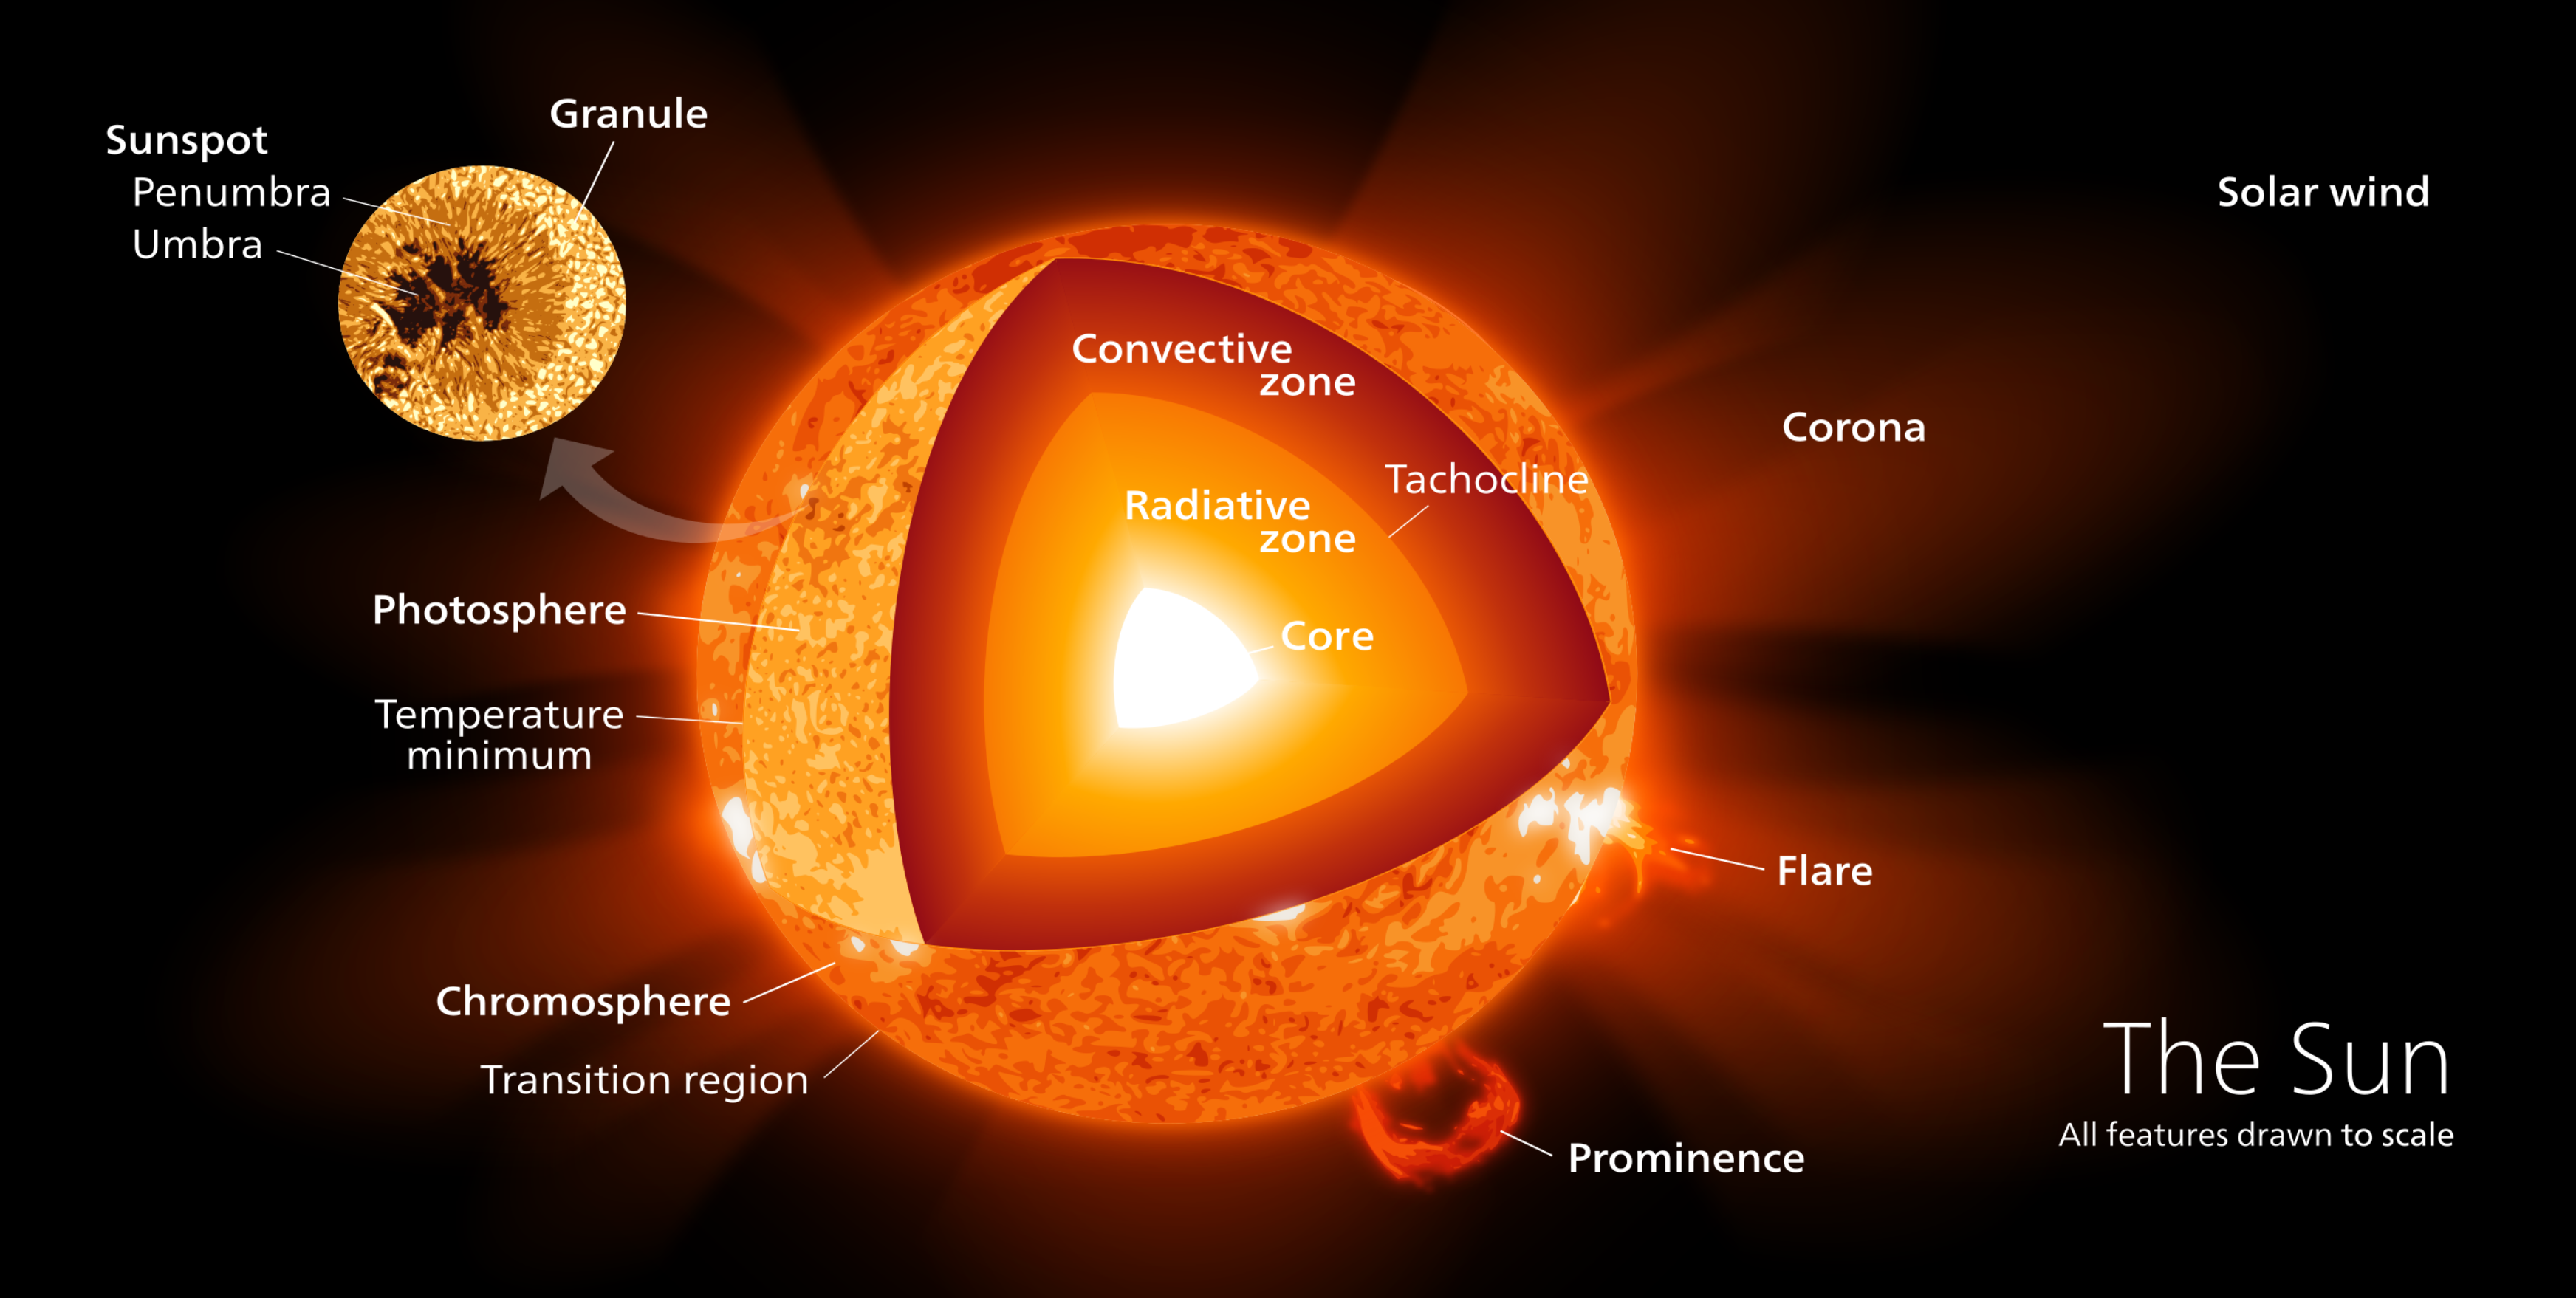
\includegraphics[width=\textwidth]{./pictures/interior.PNG}
    \caption{Visualization of the interior structure of the Sun. \cite{kelvin13}}
    \label{fig:structure}
\end{figure}
In this work we will mainly focus on phenomena related to convection, hence occurring in the convective zone and impacting photosphere.\\
Convection is the transfer of heat from one place to another by the movement of fluids. In particular, regarding the Sun, the temperature at the bottom of the convection zone is 200,000\degree K while at its outermost limit (surface of the Sun) is being cooled by the creation of light and temperature is only about 5700\degree K. This large difference triggers the plasma movement in order to propagate the heat outwards. Note, for instance, in Figure~\ref{fig:convect-cells} the bright regions correspond to hot rising material, whereas the dark lanes are the location where the colder material falls down into the Sun \cite{convect}. Also, as the reader can verify from Figure~\ref{fig:convect-cells} the way convection cells organise on the surface is not regular but rather chaotic and turbulent.
\begin{figure}[t]
    \centering
    \begin{subfigure}[b]{0.49\textwidth}
        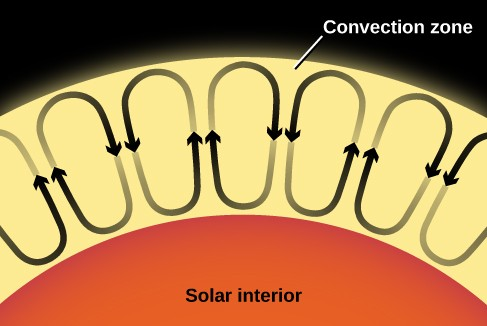
\includegraphics[width=\textwidth]{./pictures/convection}
        \caption{Section view, plasma movement}
        \label{fig:convect}
    \end{subfigure}
    \begin{subfigure}[b]{0.49\textwidth}
        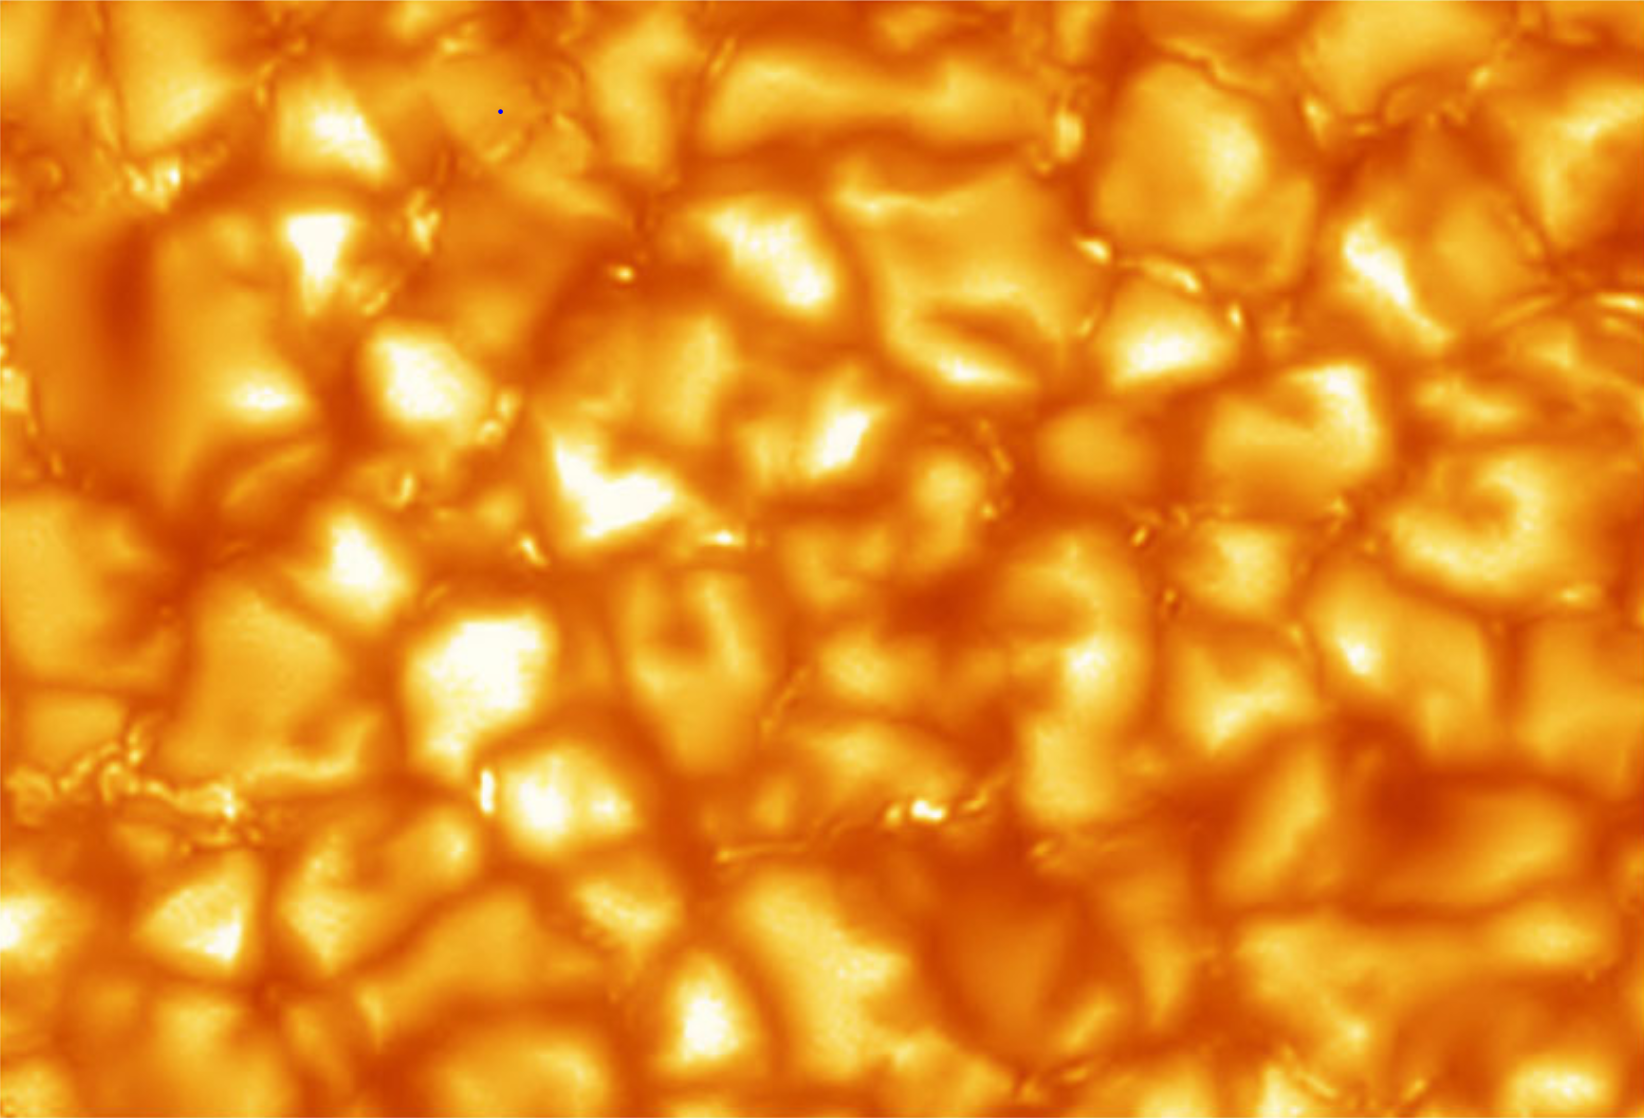
\includegraphics[width=\textwidth]{./pictures/convection-cell}
        \caption{Frontal view, convection cells.}
        \label{fig:convect-cells}
    \end{subfigure}
    \caption{Convection}\label{fig:systemview}
\end{figure}

\begin{figure}[b]
    \centering
    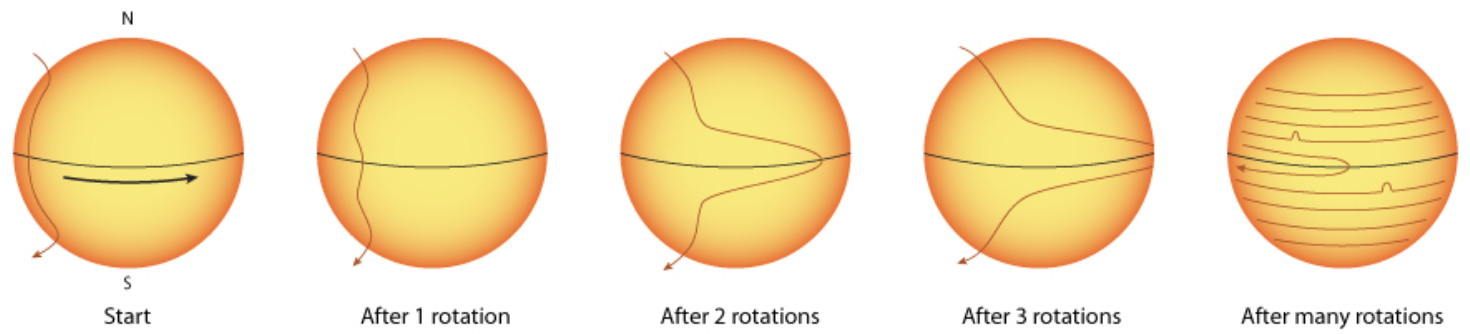
\includegraphics[width=\textwidth]{./pictures/diffrot}
    \caption{Visualization of differential rotation}
    \label{fig:diffrot}
\end{figure}
\begin{figure}[t]
    \centering
    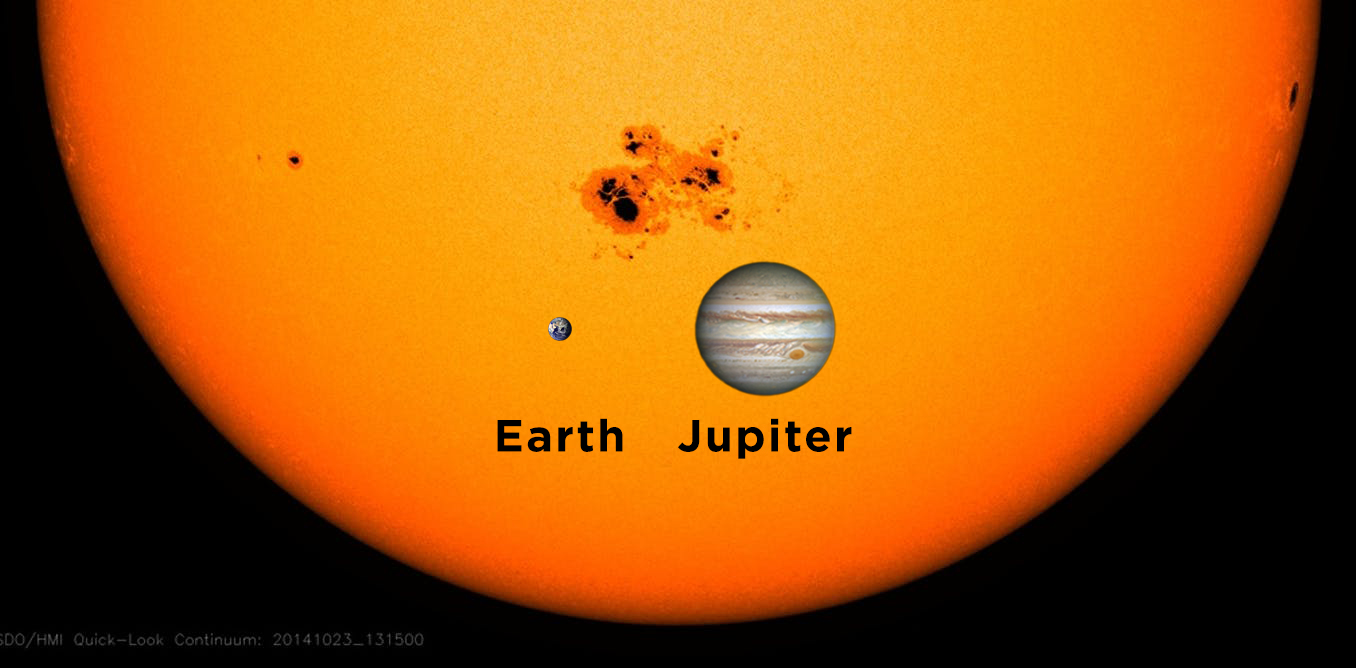
\includegraphics[width=\textwidth]{./pictures/AR12192-jup-earth}
    \caption{Relative size of AR12192, the Earth and Jupiter}
    \label{fig:AR12192-comp}
\end{figure}
Another interesting feature of the dynamics of the Sun is its rotation. In fact the sun does not rotate uniformly, since it is not a rigid object (a solid body in which deformation is zero or very small). Our star is composed of gasses in the form of plasma and therefore the relative movement of its inner particles cannot be neglected. This results in a type of motion called differential rotation. It has been observed that the angular velocity of the particles changes in a way that depends on the latitude, in particular it is fastest on the solar equator and decreases as latitude increases \cite{diffrot}. From this notion follows that the rotation period is not constant, it takes 24.47 days at the equator and almost 38 days at the poles \cite{diffrotrev}. Furthermore this behaviour has a critical importance for the understanding of this work for two reasons. First, the features that we studied are located on the photosphere and move with the surface of the Sun, undergoing significant deformation. Second, differential rotation together with convective turbulent motions leads to the generation of electric currents and solar magnetic field. This phenomenon is called solar dynamo and is in some way similar to the dynamo effect that generates the magnetic field of the Earth. Moreover the generated magnetic field has the property that it tends to agglomerate into bundles called magnetic flux tubes. When these tubes become strong enough to locally inhibit convection the heat coming from inside the Sun is not propagated upwards and the temperature of the surface decreases significantly. The local temperature drop makes the affected area look darker than the rest of the disk. These black patches, commonly named \textbf{sunspots}, can become very large and thus fairly easy to observe, even with amateur instrumentation. Their average size is comparable to the one of the Earth, but in some cases, when the magnetic perturbation is very strong, they can reach approximately the size of Jupiter or even more, as in the case of AR12192 (Figure~\ref{fig:AR12192-comp}, Figure~\ref{fig:AR12192-comp}), the largest group of the last solar cycle. Also, it has been shown that, since they indicate intense magnetic activity, sunspots accompany secondary phenomena such as coronal loops, prominences, flares and coronal mass ejections. For this reasons they have been widely observered and studied during the last 400 years. Since the invention of the telescope \cite{king2003history} (early XVII Century) many astronomers started to notice these dark features, although they weren't quite sure about their causes. Some thought they were shadows of undiscovered planets crossing the Sun, while others believed them to be dark clouds in the Sun's atmosphere. In 1843 an amateur German astronomer named Samuel Schwabe discovered the rise and fall of yearly sunspot counts we now call the solar cycle \cite{schwabe1843solar}. Nowadays we actually know that, more in general, the solar cycle is the nearly periodic 11-year change in the Sun's activity that encompasses a multitude of phenomena, as, for example, the variable levels of solar radiation and ejection of solar material. As already discussed, the change in magnitude of the activity of our star is also visible on the Earth; for instance large geomagnetic storms leading to auroras are most common during the peak of the cycle. Soon after, in 1848, Rudolf Wolf established a relative sunspot number formulation to compare the work of different astronomers using varying equipment and methodologies, known as the Wolf (or Z\"{u}rich) sunspot number \cite{vaquero2007historical}. Such definition is still in used today. Wolf succeeded in reliably reconstructing the variations in sunspot number as far as the 1755--1766 cycle, which has since been known conventionally as \textit{Cycle 1}, with all subsequent cycles numbered consecutively thereafter; at the time of writing (early 2019), we are in the final phase of \textit{Cycle 24}, although the first sunspot of \textit{Cycle 25} may have appeared in early April 2018 \cite{cycle25-1}\cite{cycle25-2} or even December 2016 \cite{cycle25-3}. Using Figure~\ref{fig:SILSO2} and Figure~\ref{fig:ssarea} the reader himself can verify that the trend is indeed periodic. Moreover the graphics highlights peaks and valleys; a peak in the sunspot count is referred to as a time of \textit{solar maximum}, whereas a valley, a period when just few sunspots appear is called a \textit{solar minimum}.
\begin{figure}[t]
    \centering
    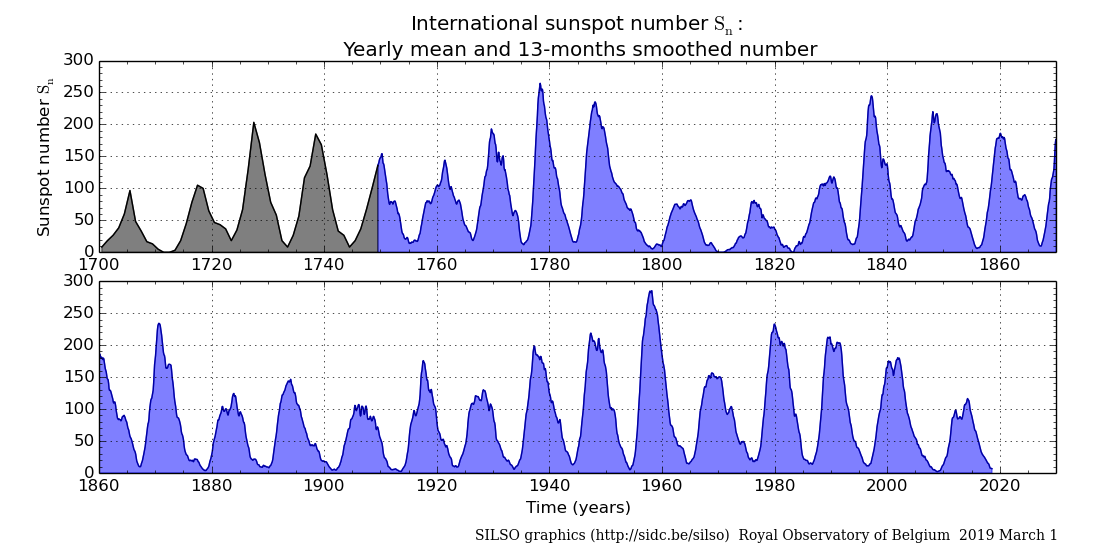
\includegraphics[width=\textwidth]{./pictures/SILSO2}
    \caption{Yearly mean sunspot number (black) up to 1749 and monthly 13-month smoothed sunspot number (blue) from 1749 up to the present.\cite{silso-graph}}
    \label{fig:SILSO2}
\end{figure}
Focusing on Figure~\ref{fig:butterfly}, instead we can discover another peculiar feature of the sunspot cycle: \textit{Sp\"{o}rer's law} \cite{ivanov2014sporer}. Sp\"{o}rer's law predicts the variation of sunspot position during a solar cycle. He introduced the concept of \textit{cycle latitude phase} (CLP), which is calculated from the behavior of average latitudes. In particular, sunspots tend to appear around 30\degree  to 45\degree  latitude on the Sun's surface. As the cycle progresses, sunspots appear at lower and lower latitudes, until they average 15\degree  at solar maximum. The average latitude of sunspots then continues to drift lower, down to about 7\degree  and then while the old sunspot cycle fades, sunspots of the new cycle start appearing at high latitudes.
\begin{figure}[t]
    \centering
    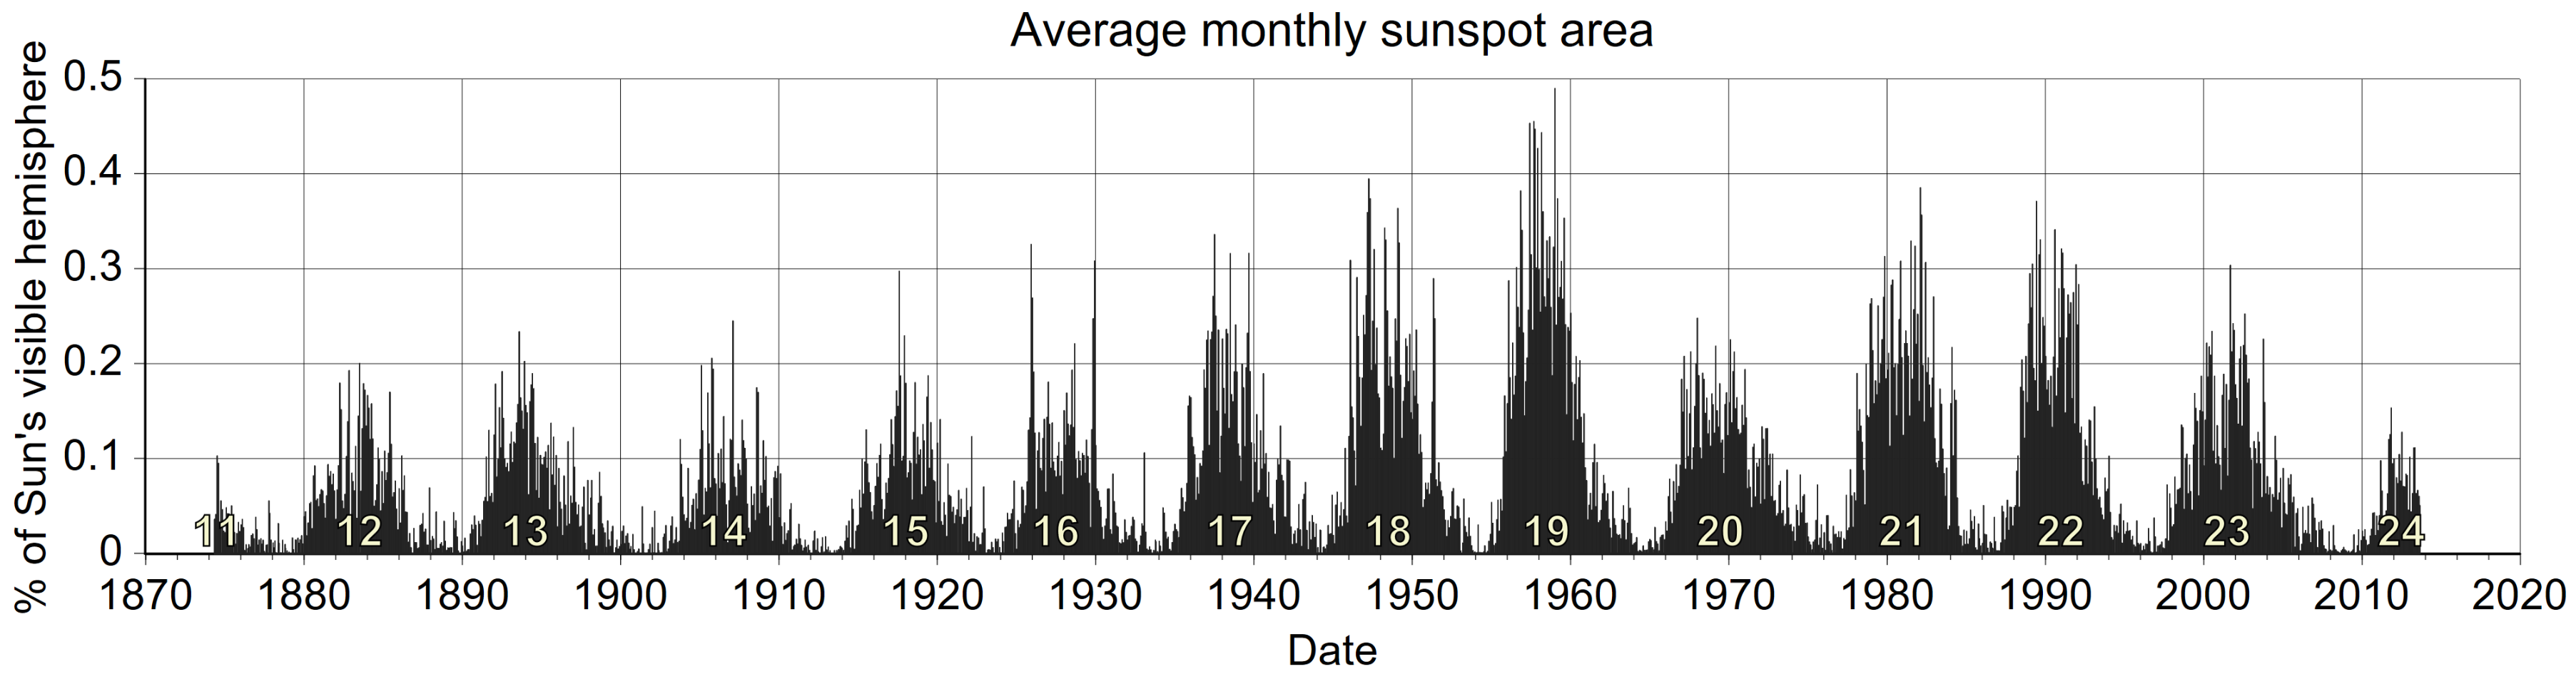
\includegraphics[width=\textwidth]{./pictures/ssarea}
    \caption{Diagram showing average monthly sunspot area from cycle 12 to cycle 24}
    \label{fig:ssarea}
\end{figure}
\begin{figure}[t]
    \centering
    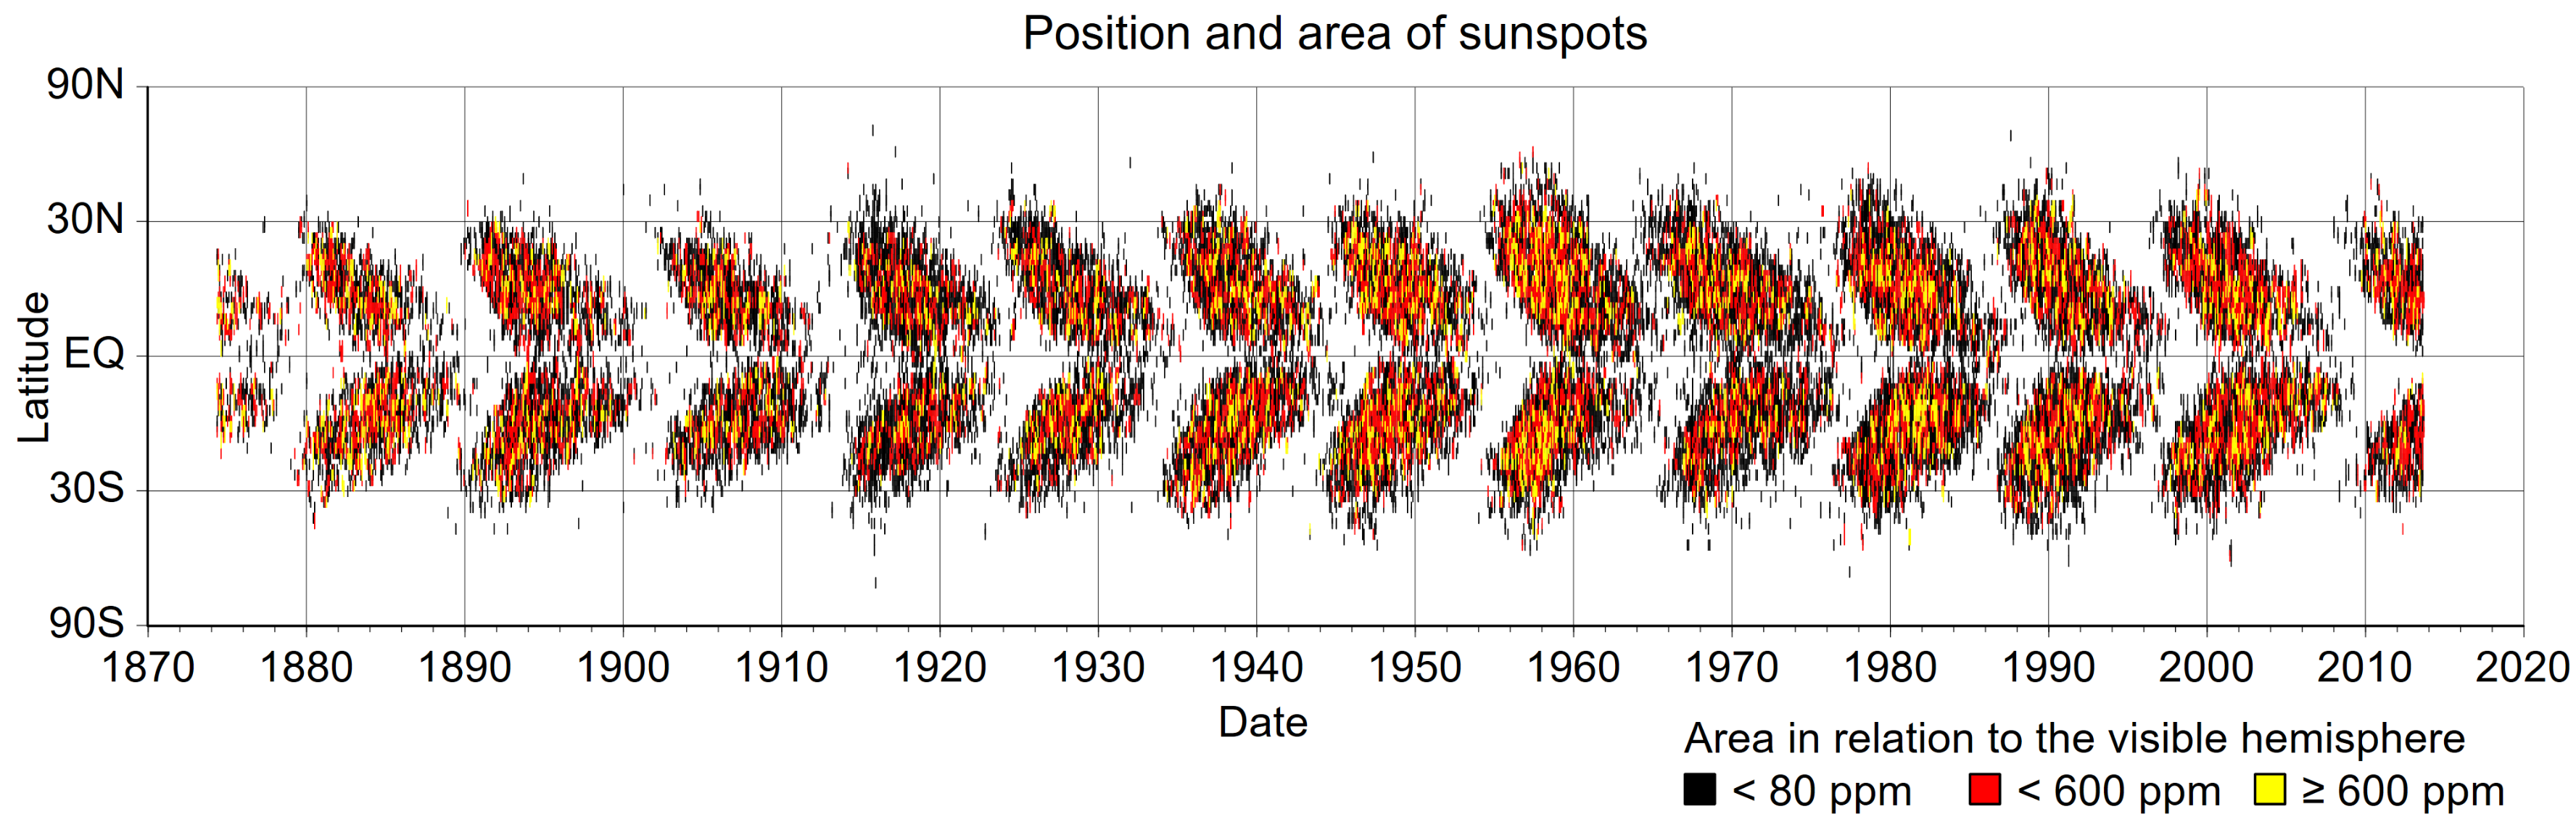
\includegraphics[width=\textwidth]{./pictures/butterfly}
    \caption{Butterfly diagram showing paired position and area of sunspots}
    \label{fig:butterfly}
\end{figure}
The last notion we need to introduce in order for the reader to fully understand this work is sunspot classification. Several different categorization paradigms have been introduced during the years but the one that is most popular nowadays is the \textit{McIntosh classification}, introduced in 1990 \cite{mcintosh1990classification}. The McIntosh classification is constituted by three components, in which the nomenclature used for each sunspot group type is \textbf{Zpc}, where Z corresponds to \textit{Modified Z\"{u}rich Classification}, and the other two components, p and c, reflect the main sunspot characteristics: the type, size, and symmetry of the penumbra and umbra; and the degree of compactness of the group \cite{carrasco2015equivalence}. We will focus on the \textbf{Z} component, that divides the spots in the following categories\cite{}:
\begin{itemize}
  \item \textbf{A}: a small single unipolar sunspot. Representing either the formative or final stage of evolution;
  \item \textbf{B}: a bipolar sunspot group with no penumbra on any of the spots;
  \item \textbf{C}: a bipolar sunspot group. One sunspot must have penumbra;
  \item \textbf{D}: a bipolar sunspot group with penumbra on both ends of the group. Longitudinal extent does not exceeds 10 deg;
  \item \textbf{E}: a bipolar sunspot group with penumbra on both ends. Longitudinal extent exceeds 10 deg. but not 15 deg;
  \item \textbf{F}: an elongated bipolar sunspot group with penumbra on both ends. Longitudinal extent of penumbra exceeds 15 deg;
  \item \textbf{H}: a unipolar sunspot group with penumbra.
\end{itemize}






% \begin{figure}[b]
%     \centering
%     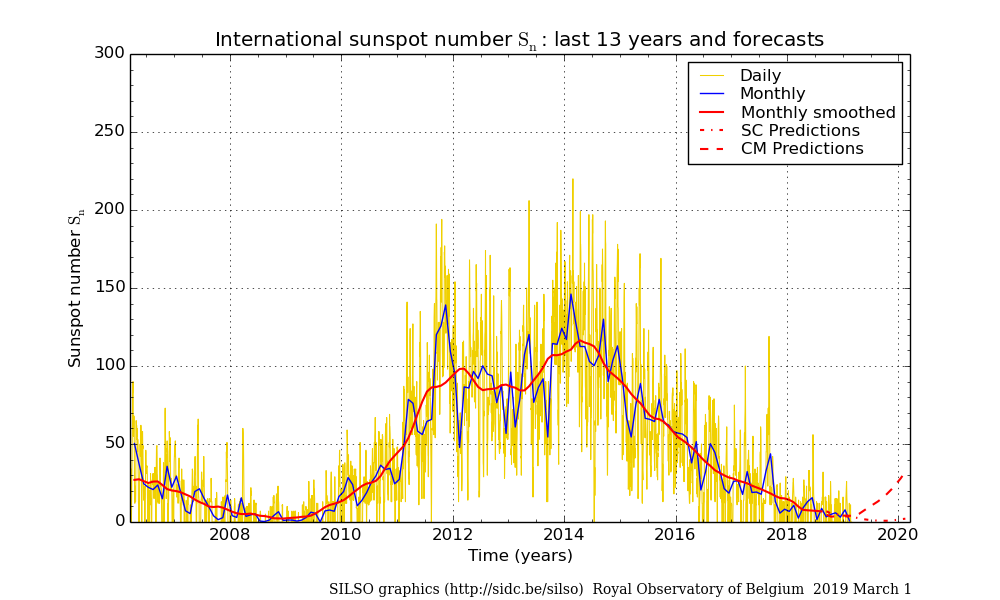
\includegraphics[width=\textwidth]{./pictures/SILSO1}
%     \caption{Daily sunspot number (yellow), monthly mean sunspot number (blue), smoothed monthly sunspot number (red) for the last 13 years and 12-month ahead predictions of the monthly smoothed sunspot number. SC = prediction method based on an interpolation of Waldmeier's standard curves. CM = method (from K. Denkmayr and P. Cugnon) combining a regression technique applied to the sunspot number series with the a geomagnetic index used as a precursor}
%     \label{fig:SILSO1}
% \end{figure}
%
%
% \begin{figure}[t]
%     \centering
%     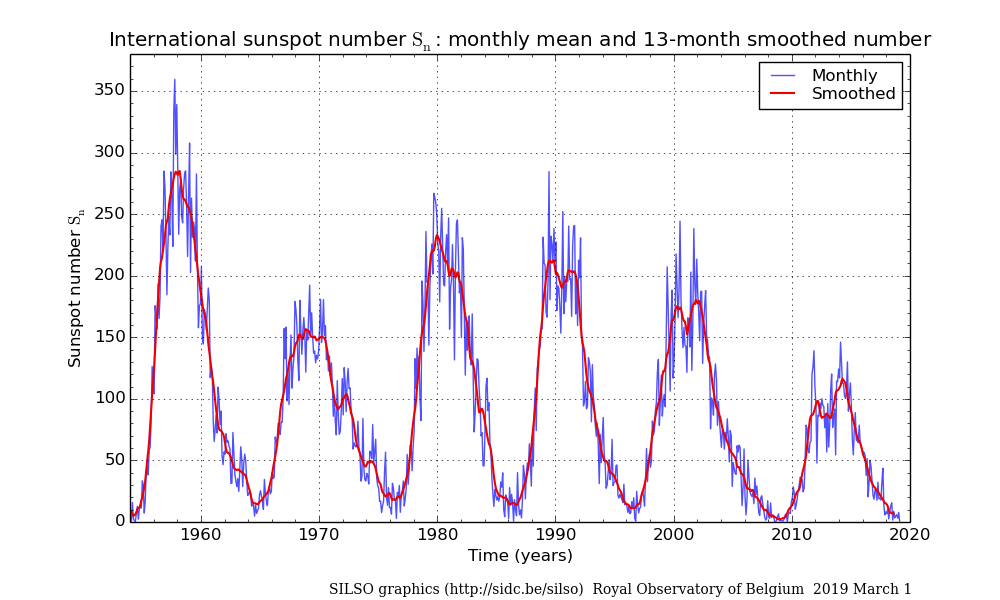
\includegraphics[width=\textwidth]{./pictures/SILSO3}
%     \caption{The monthly mean sunspot number (blue) and 13-month smoothed monthly sunspot number (red) for the last five cycles.}
%     \label{fig:SILSO3}
% \end{figure}

% \begin{figure}[t]
%     \centering
%     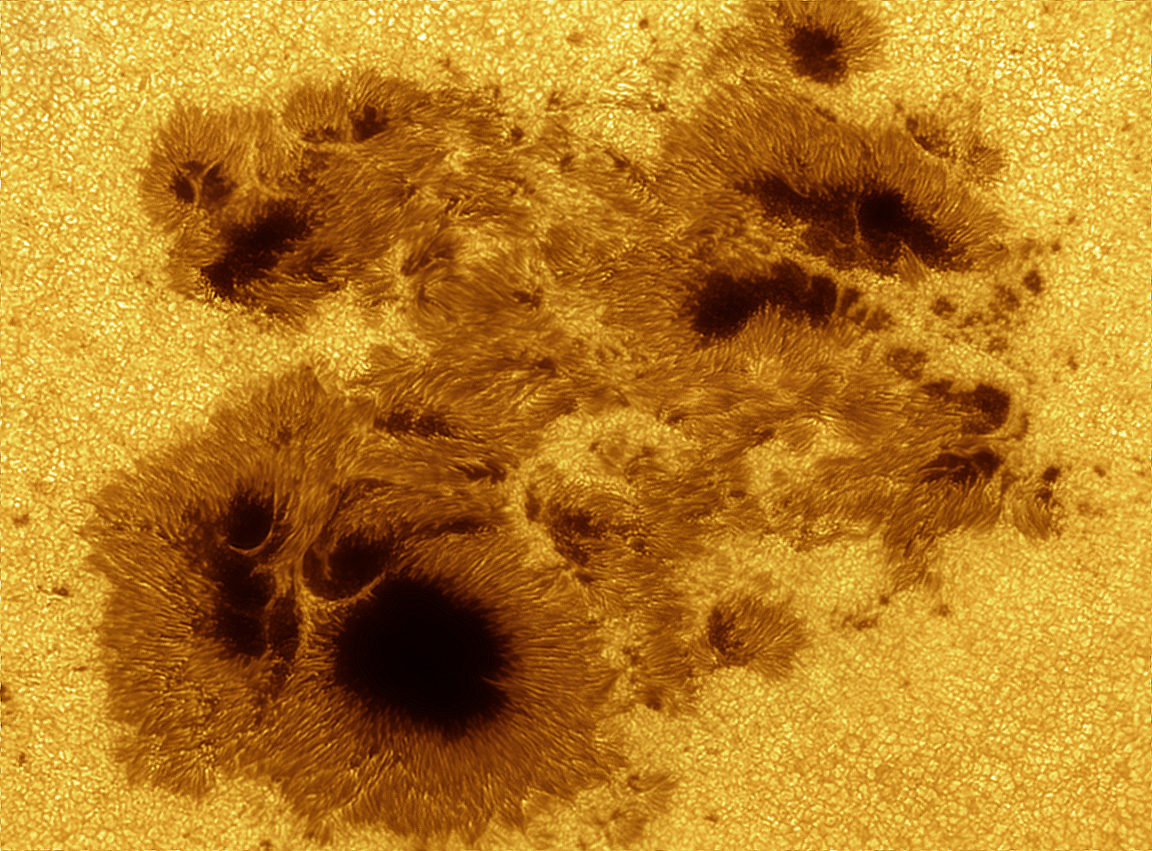
\includegraphics[width=\textwidth]{./pictures/AR12192}
%     \caption{Close up picture of AR12192}
%     \label{fig:AR12192}
% \end{figure}
